\clearpage
\phantomsection
\vspace*{0.2cm}

مبانی نظری این معماری مبتنی بر دستاوردهای علمی \cite{ref_asvdattention_2024} است.
\noindent\rule{\textwidth}{1.2pt}
\vspace*{0.1cm}
\section{تحلیل علمی و کالبدشکافی ساختاری ماژول \lr{asvd\_attention}}
\label{sec:mod_asvd_attention}
\vspace*{-0.2cm}
\noindent\rule{\textwidth}{0.5pt}
\vspace*{0.3cm}

\subsection*{بخش ۱: ایده محوری و چرایی معماری \lr{(Architectural Rationale)}}
مکانیزم توجه چندسره استاندارد \lr{(Standard Multi-Head Attention - MHA)} سنگ‌بنای مدل‌های زبانی بزرگ است؛ با این وجود، تشکیل ماتریس‌های وزن پروجکشن متراکم $\mathbf{W}_Q, \mathbf{W}_K, \mathbf{W}_V, \mathbf{W}_O \in \mathbb{R}^{D \times D}$ بار محاسباتی و ردپای حافظه‌ای عظیمی را بر زیرساخت سخت‌افزاری تحمیل می‌نماید. در مدل‌های سنتی تقلیل رتبه مبتنی بر تجزیه مقادیر منفرد \lr{(Truncated Singular Value Decomposition - SVD)}، ماتریس وزن ایستا صرفاً بر پایه اندازه عددی درایه‌های وزن فاکتورگیری شده و فرض بنیادین بر توزیع نرمال و همسانگرد \lr{(Isotropic)} فعال‌سازی‌های ورودی ($\mathbf{X} \sim \mathcal{N}(0, \mathbf{I})$) استوار است.

تحقیقات عمیق سال‌های اخیر بر رفتار پنهان مدل‌های زبانی آشکار ساخته است که فعال‌سازی‌های پنهان درون لایه‌های ترنسفورمر دارای توزیع به شدت ناهمگن با چگالی طیفی ناهمسانگرد هستند. پدیده کانال‌های پرت \lr{(Activation Outliers)} نشان می‌دهد که کمتر از \lr{0.5\%} از کانال‌های ابعاد پنهان، مقادیری تا ۱۰۰ برابر بزرگتر از کانال‌های معمول به خود اختصاص می‌دهند. هنگام اعمال تقریب کم‌مرتبه بدون توجه به فعال‌سازی‌ها، خطای بازسازی خروجی لایه به صورت $\|(\mathbf{W} - \mathbf{W}_r)\mathbf{X}^\top\|_F$ فرمول‌بندی می‌شود. در صورتی که پایه‌های متعامد مقادیر منفرد ماتریس وزن بر راستای کانال‌های پرت منطبق نباشند، خطاهای جزیی وزن در راستای این کانال‌ها با ضریب $10^4$ در فضای توان تشدید شده و به فروپاشی فاحش بیانی و معنایی مدل منجر می‌گردند.

مکانیزم توجه آگاه از فعال‌سازی \lr{(Activation-Aware Singular Value Decomposition Attention - ASVD)} این پارادوکس را از طریق بهینه‌سازی توزیع مقادیر منفرد بر پایه ماتریس کوواریانس فعال‌سازی حل می‌کند. ایده محوری ماژول \lr{asvd\_attention}، بازتعریف مسئله تقریب کم‌مرتبه از فضای استاتیک وزن به فضای دینامیک انتقال فعال‌سازی است:
\begin{equation}
\min_{\operatorname{rank}(\hat{\mathbf{W}}) \le r} \mathbb{E}_{\mathbf{X}}\left[ \|\mathbf{X}\mathbf{W}^\top - \mathbf{X}\hat{\mathbf{W}}^\top\|_F^2 \right] = \min_{\operatorname{rank}(\hat{\mathbf{W}}) \le r} \|(\mathbf{W} - \hat{\mathbf{W}})\mathbf{C}_X^{1/2}\|_F^2
\end{equation}
که در آن $\mathbf{C}_X = \frac{1}{N}\mathbf{X}^\top \mathbf{X}$ ماتریس کوواریانس تجربی فعال‌سازی‌ها است. با پیش‌سفیدسازی \lr{(Pre-whitening)} ماتریس وزن از طریق ضرب در ریشه کوواریانس فعال‌سازی ($\mathbf{M} = \mathbf{W}\mathbf{C}_X^{1/2}$)، تجزیه طیفی مستقیماً بر جهات با واریانس انرژی حداکثری قفل شده و حساس‌ترین کانال‌های معنایی مدل حفظ می‌شوند.

علاوه بر این، ماژول \lr{asvd\_attention} ساختار سه‌عاملی صریحی را با تفکیک پایه‌های راست و چپ ($\mathbf{U}, \mathbf{V}$)، بردار مقیاس‌گذاری مقادیر منفرد ($\mathbf{S}$)، و مسیر موازی سازگارکننده کم‌مرتبه با رتبه پایین \lr{(Low-Rank Adaptation - LoRA)} معرفی می‌نماید. در این طراحی، پس از فاکتورسازی اولیه، پایه‌های اصلی منجمد \lr{(Frozen)} گشته و صرفاً بردارهای مقیاس و آداپتورهای \lr{LoRA} در طول فاز بازیافت دقیق کالیبره می‌شوند. این استراتژی ضمن جلوگیری از پراکندگی گرادیان‌ها در محاسبات نیم‌دقت، بیش از \lr{91.6\%} از پارامترهای پروجکشن لایه توجه را حذف کرده و عملکردی قابل توجه سریع بر روی پردازنده‌های گرافیکی تجاری ثبت می‌کند.

\subsection*{بخش ۲: فرمول‌بندی ریاضی و مبانی نظری \lr{(Mathematical Formulation)}}
فرض کنید تانسور نمایش پنهان ورودی به لایه توجه با ابعاد $\mathbf{X} \in \mathbb{R}^{B \times N \times D}$ داده شده باشد، که در آن $B$ اندازه دسته \lr{(Batch Size)}، $N$ طول توالی \lr{(Sequence Length)} و $D$ بعد پنهان مدل \lr{(Hidden Dimension)} است. پروجکشن‌های استاندارد خطی عبارتند از:
\begin{equation}
\mathbf{Q} = \mathbf{X}\mathbf{W}_Q, \quad \mathbf{K} = \mathbf{X}\mathbf{W}_K, \quad \mathbf{V} = \mathbf{X}\mathbf{W}_V, \quad \mathbf{O} = \mathbf{C}\mathbf{W}_O
\end{equation}
که در آن‌ها $\mathbf{W}_Q \in \mathbb{R}^{D \times D_{\text{\lr{all}}}}$, $\mathbf{W}_K, \mathbf{W}_V \in \mathbb{R}^{D \times D_{KV}}$, $\mathbf{W}_O \in \mathbb{R}^{D_{\text{\lr{all}}} \times D}$ با $D_{\text{\lr{all}}} = H \cdot d$ و $D_{KV} = H_{KV} \cdot d$ تعریف می‌شوند ($H$ تعداد سرهای پرس‌وجو، $H_{KV}$ تعداد سرهای کلید/مقدار، و $d = D/H$ بعد اختصاصی هر سر).

\subsubsection*{قضیه اکارت-یانگ-میرسکی و تقریب کم‌مرتبه \lr{(Eckart-Young-Mirsky Theorem)}}
بر اساس قضیه اکارت-یانگ-میرسکی، برای هر ماتریس $\mathbf{W} \in \mathbb{R}^{d_{\text{\lr{out}}} \times d_{\text{\lr{in}}}}$ با تجزیه مقادیر منفرد کامل $\mathbf{W} = \mathbf{U}\mathbf{\Sigma}\mathbf{V}^\top = \sum_{i=1}^{\min(d_{\text{\lr{out}}}, d_{\text{\lr{in}}})} \sigma_i \mathbf{u}_i \mathbf{v}_i^\top$ (که $\sigma_1 \ge \sigma_2 \ge \dots \ge 0$ مقادیر منفرد مرتب‌شده هستند)، بهینه‌ترین تقریب رتبه-$r$ ماتریسی تحت هر دو نُرم فروبنیوس و طیفی برابر است با:
\begin{equation}
\mathbf{W}_r = \arg\min_{\operatorname{rank}(\hat{\mathbf{W}}) \le r} \|\mathbf{W} - \hat{\mathbf{W}}\|_F = \sum_{i=1}^r \sigma_i \mathbf{u}_i \mathbf{v}_i^\top
\end{equation}
با کران خطای دقیق بازسازی:
\begin{equation}
\|\mathbf{W} - \mathbf{W}_r\|_F = \sqrt{\sum_{j=r+1}^{\min(d_{\text{\lr{out}}}, d_{\text{\lr{in}}})} \sigma_j^2}, \qquad \|\mathbf{W} - \mathbf{W}_r\|_2 = \sigma_{r+1}
\end{equation}

\subsubsection*{تحلیل ریاضی توزیع متقارن مقادیر منفرد و مهار گرادیان در \lr{FP16}}
در پیاده‌سازی لایه‌های کم‌مرتبه $y = (x \mathbf{V}^\top)\mathbf{U}^\top$، تخصیص نامتقارن مقادیر منفرد به یکی از پایه‌ها (مثلاً $\mathbf{U} = \mathbf{U}_r \mathbf{\Sigma}_r$ و $\mathbf{V} = \mathbf{V}_r$) موجب عدم توازن شدید در نرم گرادیان‌ها در فاز پس‌انتشار می‌گردد:
\begin{align}
\nabla_{\mathbf{V}} \mathcal{L} &= \mathbf{U}^\top \boldsymbol{\delta}_y^\top \mathbf{x} \implies \|\nabla_{\mathbf{V}} \mathcal{L}\|_F \le \|\mathbf{U}\|_2 \|\boldsymbol{\delta}_y\|_F \|\mathbf{x}\|_F = \sigma_1 \|\boldsymbol{\delta}_y\|_F \|\mathbf{x}\|_F \\
\nabla_{\mathbf{U}} \mathcal{L} &= \boldsymbol{\delta}_y^\top (\mathbf{x} \mathbf{V}^\top) \implies \|\nabla_{\mathbf{U}} \mathcal{L}\|_F \le \|\mathbf{V}\|_2 \|\boldsymbol{\delta}_y\|_F \|\mathbf{x}\|_F = 1 \cdot \|\boldsymbol{\delta}_y\|_F \|\mathbf{x}\|_F
\end{align}
از آنجا که در شبکه‌های عمیق مقدار منفرد غالب $\sigma_1 \sim 10^2 - 10^3$ است، در محاسبات ممیز شناور نیم‌دقت \lr{(FP16)} که سقف مقادیر مجاز $65504$ و مرز تقریب صفر $\approx 6.1 \times 10^{-5}$ است، مربعات گرادیان در بهینه‌سازهای تطبیقی ($\nabla_{\mathbf{V}}^2 \sim \sigma_1^2 \sim 10^6$) بلادرنگ دچار سرریز \lr{(Overflow)} و تولید مقادیر \lr{NaN/Inf} می‌گردند، در حالی که گرادیان $\nabla_{\mathbf{U}}$ دچار زیرریز \lr{(Underflow)} می‌شود.

ماژول \lr{asvd\_attention} با تفکیک صریح بردار مقادیر منفرد $\mathbf{S} \in \mathbb{R}^r$ میان دو پایه کاملاً یکانی $\mathbf{U}^\top \mathbf{U} = \mathbf{I}_r$ و $\mathbf{V}\mathbf{V}^\top = \mathbf{I}_r$، عدد حالت عملگر را در مقیاس لگاریتمی به نصف تقلیل می‌دهد:
\begin{equation}
\kappa(\mathbf{U}) = 1, \quad \kappa(\mathbf{V}) = 1, \quad \frac{\|\nabla_{\mathbf{V}} \mathcal{L}\|_F}{\|\nabla_{\mathbf{U}} \mathcal{L}\|_F} = 1.0
\end{equation}
این برابری دینامیکی، تعادل کامل بازگشت گرادیان را در فرمت \lr{FP16/BF16} تضمین می‌نماید.

\subsubsection*{فرمول‌بندی عملگر خطی فاکتورگیری‌شده \lr{ASVDLinear}}
تبدیل پروجکشن هر توکن $\mathbf{x} \in \mathbb{R}^{d_{\text{\lr{in}}}}$ به خروجی $\mathbf{y} \in \mathbb{R}^{d_{\text{\lr{out}}}}$ در لایه \lr{ASVDLinear} به صورت فرمول‌بندی زیر اجرا می‌شود:
\begin{equation}
\mathbf{y} = \left( \left( \mathbf{x} \mathbf{V}^\top \right) \odot \mathbf{S} \right) \mathbf{U}^\top + \frac{\alpha}{r_{\text{\lr{lora}}}} \left( \mathbf{x} \mathbf{A}^\top \right) \mathbf{B}^\top + \mathbf{b}
\end{equation}
که در آن:
\begin{itemize}
    \item $\mathbf{V} \in \mathbb{R}^{r \times d_{\text{\lr{in}}}}$: پایه متعامد پروجکشن به زیرفضای فشرده،
    \item $\mathbf{S} \in \mathbb{R}^r$: بردار مقادیر منفرد مقیاس‌پذیر،
    \item $\mathbf{U} \in \mathbb{R}^{d_{\text{\lr{out}}} \times r}$: پایه متعامد بازسازی ابعاد خروجی،
    \item $\mathbf{A} \in \mathbb{R}^{r_{\text{\lr{lora}}} \times d_{\text{\lr{in}}}}$ و $\mathbf{B} \in \mathbb{R}^{d_{\text{\lr{out}}} \times r_{\text{\lr{lora}}}}$: پارامترهای آموزش‌پذیر آداپتور \lr{LoRA} با ضریب مقیاس $\alpha$،
    \item $\mathbf{b} \in \mathbb{R}^{d_{\text{\lr{out}}}}$: بردار بایاس پروجکشن.
\end{itemize}

\subsubsection*{انتخاب پویای رتبه بر مبنای آستانه انرژی تراکمی \lr{(Cumulative Energy)}}
به جای استفاده از رتبه ثابت، رتبه موثر $r$ برای هر پروجکشن بر اساس آستانه انرژی تراکمی طیف مقادیر منفرد با رابطه توانی $\sigma_i \approx i^{-\beta}$ با ضریب $\beta \approx 0.85$ به صورت پویا تعیین می‌گردد:
\begin{equation}
\mathcal{E}(r) = \frac{\sum_{i=1}^r \sigma_i^2}{\sum_{j=1}^{\min} \sigma_j^2} \ge \tau \quad (\tau = 0.95)
\end{equation}
کران بالای خطای واریانس خروجی برای توزیع ورودی با کوواریانس $\mathbf{\Sigma}_X$ عبارت است از:
\begin{equation}
\mathbb{E}_{\mathbf{x}}\left[\|\mathbf{W}\mathbf{x} - \mathbf{W}_r \mathbf{x}\|_2^2\right] \le \lambda_{\max}(\mathbf{\Sigma}_X) (1 - \tau) \|\mathbf{W}\|_F^2 = 0.05 \cdot \lambda_{\max}(\mathbf{\Sigma}_X) \|\mathbf{W}\|_F^2
\end{equation}
این کران تضمین می‌کند که خطای بازسازی زیرفضایی لایه از آستانه پایداری لایه‌های نرمال‌سازی بعدی فراتر نرود.

\subsubsection*{تحلیل پیچیدگی محاسباتی و حافظه}
پیچیدگی محاسباتی پروجکشن‌های لایه توجه از $\mathcal{O}(B \cdot N \cdot D^2)$ به $\mathcal{O}(B \cdot N \cdot r \cdot D)$ کاهش می‌یابد. پیچیدگی محاسبات ماتریس شباهت و وزن‌دهی توجه در فرمول استاندارد در دقت ممیز شناور کامل برابر با $\mathcal{O}(B \cdot H \cdot N^2 \cdot d)$ باقی می‌ماند. بنابراین، پیچیدگی زمانی کل لایه برابر است با:
\begin{equation}
\mathcal{T}_{\text{\lr{total}}} = \mathcal{O}\left( B \cdot N \cdot r \cdot D + B \cdot H \cdot N^2 \cdot d \right)
\end{equation}
پیچیدگی حافظه پارامتری از $\mathcal{O}(4 D^2)$ به $\mathcal{O}(4 \cdot (2 r D + r + 2 r_{\text{\lr{lora}}} D))$ تنزل یافته که به معنای صرفه‌جویی خطی عظیمی در اشغال حافظه وزن‌ها است.

\subsection*{بخش ۳: کالبدشکافی سورس‌کد و ردگیری تانسورها \lr{(Source Code \& Tensor Trace)}}
ماژول \lr{asvd\_attention} در قالب کلاس اصلی \lr{ASVDAttention} و کلاس پایه تبدیل خطی کم‌مرتبه \lr{ASVDLinear} پیاده‌سازی شده و در رجیستری مرکزی با برچسب‌های \lr{"asvd"} و \lr{"asvd\_attention"} ثبت گردیده است. این ماژول به طور بومی از ماسک‌گذاری علّی \lr{(Causal Masking)}، توجه دوسویه انکودر، توجه با سرهای گروه‌بندی‌شده \lr{(GQA)} و کدگذاری مکانی چرخشی \lr{(RoPE)} پشتیبانی می‌نماید.

\subsubsection*{سلسله‌مراتب کلاسی و تفکیک لایه‌ها}
کلاس \lr{ASVDLinear} وظیفه اجرای تبدیل سه‌عاملی را با تعریف پارامترهای $\mathbf{U}$، $\mathbf{S}$، $\mathbf{V}$، بایاس و آداپتورهای \lr{LoRA} برعهده دارد. متد \lr{reset\_parameters} مقادیر $\mathbf{U}$ و $\mathbf{V}$ را به صورت پایه‌های متعامد \lr{(Orthogonal Initialization)} مقداردهی اولیه کرده، درایه‌های $\mathbf{S}$ را با مقدار یک پر می‌کند، ماتریس $\mathbf{A}$ آداپتور \lr{LoRA} را با توزیع یکنواخت کایمینگ و ماتریس $\mathbf{B}$ را با صفر مقداردهی می‌نماید. با فراخوانی \lr{freeze\_base\_weights()}، گرادیان پارامترهای پایه قطع گردیده و تنها آداپتورها در طول فرآیند بازیافت بهینه‌سازی می‌شوند.

\subsubsection*{ردگیری تانسورها در متد پیشرو \lr{(Forward Pass)}}
تانسور ورودی $\mathbf{X} \in \mathbb{R}^{B \times N \times D}$ مراحل محاسباتی زیر را به ترتیب طی می‌کند:
\begin{enumerate}
    \item \textbf{پروجکشن کم‌مرتبه پرس‌وجو، کلید و مقدار:}
    \begin{align}
    \mathbf{Q}_{\text{\lr{flat}}} &= \text{\lr{self.query}}(\mathbf{X}) \in \mathbb{R}^{B \times N \times (H \cdot d)} \\
    \mathbf{K}_{\text{\lr{flat}}} &= \text{\lr{self.key}}(\mathbf{X}) \in \mathbb{R}^{B \times N \times (H_{KV} \cdot d)} \\
    \mathbf{V}_{\text{\lr{flat}}} &= \text{\lr{self.value}}(\mathbf{X}) \in \mathbb{R}^{B \times N \times (H_{KV} \cdot d)}
    \end{align}
    تانسورها به ساختار چندسره تغییر ابعاد داده و ترانهاده می‌شوند:
    \begin{equation}
    \mathbf{Q} \in \mathbb{R}^{B \times H \times N \times d}, \quad \mathbf{K}, \mathbf{V} \in \mathbb{R}^{B \times H_{KV} \times N \times d}
    \end{equation}
    \item \textbf{اعمال کدگذاری مکانی چرخشی جزئی \lr{(Partial RoPE)}:}
    برای مدل‌های پیشرفته دیکودر نظیر سری \lr{Qwen3.5}، ابعاد چرخش $d_{\text{\lr{rot}}}$ ممکن است کوچکتر از کل بعد سر $d$ باشد ($d_{\text{\lr{rot}}} \le d$). متد \lr{apply\_rotary\_pos\_emb} مختصات چرخشی را از مختصات بدون چرخش تفکیک کرده، نگاشت چرخش را بر درایه‌های متناظر اعمال نموده و مجدداً آنها را الحاق می‌کند:
    \begin{equation}
    \mathbf{q}_{\text{\lr{rot}}} = (\mathbf{q}_{:, :, :, :d_{\text{\lr{rot}}}} \odot \cos) + (\text{\lr{\_rotate\_half}}(\mathbf{q}_{:, :, :, :d_{\text{\lr{rot}}}}) \odot \sin)
    \end{equation}
    \item \textbf{توسعه سرهای کلید و مقدار در معماری \lr{GQA}:}
    در صورت کمتر بودن تعداد سرهای کلید و مقدار نسبت به پرس‌وجو ($H_{KV} < H$)، متد \lr{repeat\_kv} با ضریب تکرار $H / H_{KV}$، ابعاد تانسورهای $\mathbf{K}$ و $\mathbf{V}$ را به $[B, H, N, d]$ گسترش می‌دهد.
    \item \textbf{محاسبه امتیازات توجه در دقت ممیز شناور کامل \lr{(FP32 Attention Scoring)}:}
    به منظور جلوگیری از خطای سرریز محاسباتی در ممیز شناور نیم‌دقت، ضرب تانسوری $\mathbf{Q} \mathbf{K}^\top$ در دقت \lr{FP32} انجام می‌شود:
    \begin{equation}
    \mathbf{S} = \frac{\mathbf{Q}_{\text{\lr{FP32}}} \mathbf{K}_{\text{\lr{FP32}}}^\top}{\sqrt{d}} \in \mathbb{R}^{B \times H \times N \times N}
    \end{equation}
    \item \textbf{ماسک‌گذاری علّی و پدینگ:}
    در سناریوهای دیکودر خودبازگشت، ماسک مثلثی بالای ماتریس با مقدار عددی $-10000.0$ افزوده می‌شود. ماسک‌های پدینگ ورودی نیز با پخشدگی دو‌بعدی و سه‌بعدی به ساختار ۴ بعدی لاجیت افزوده می‌شوند.
    \item \textbf{سافت‌مکس و محافظت در برابر \lr{NaN}:}
    توزیع توجه با تابع سافت‌مکس استخراج شده و با فراخوانی \lr{torch.nan\_to\_num(attn, nan=0.0)} پایداری کامل ماتریس احتمالات در برابر ناپایداری‌های عددی تضمین می‌گردد.
    \item \textbf{تلفیق بافت و تجمیع سرها \lr{(Context Aggregation)}:}
    ضرب بافت $\mathbf{C} = \mathbf{A} \mathbf{V} \in \mathbb{R}^{B \times H \times N \times d}$ محاسبه شده، به ساختار $[B, N, H \cdot d]$ تغییر شکل داده و با فراخوانی \lr{.contiguous()} در حافظه پیوسته می‌شود.
    \item \textbf{پروجکشن نهایی و حل پاتولوژی انکودرهای تودرتو \lr{(Nested Encoder Pathology)}:}
    در مدل‌های انکودر متداول نظیر \lr{RoBERTa}، ماژول توجه درون یک ساختار تودرتو شامل \lr{RobertaSelfAttention} و لایه بیرونی \lr{RobertaSelfOutput (output.dense)} قرار دارد. جایگزینی کورکورانه لایه توجه منجر به اعمال دو برابری پروجکشن خروجی ($\mathbf{W}_O \cdot \mathbf{W}_{\text{\lr{dense}}}$) و افت شدید نُرم خروجی به یک‌دهم می‌گردید. ماژول \lr{asvd\_attention} به طور خودکار انکودرهای تودرتو را شناسایی کرده و با فعال‌سازی پرچم \lr{is\_nested\_encoder}، پروجکشن \lr{out\_proj} را خنثی ساخته یا مستقیماً تانسور بافت را بازمی‌گرداند. در سایر مدل‌ها، پروجکشن فاکتورگیری‌شده خروجی به شکل زیر اجرا می‌شود:
    \begin{equation}
    \mathbf{O} = \text{\lr{self.out\_proj}}(\mathbf{C}) \in \mathbb{R}^{B \times N \times D}
    \end{equation}
\end{enumerate}

جدول \ref{tab:tensor_trace_asvd} ردگیری ابعاد تانسورها را در مراحل مختلف برای طول دنباله ۱۲۸ و بعد پنهان ۷۶۸ با رتبه فشرده‌سازی $r=32$ نمایش می‌دهد.

\begin{table}[H]
\centering
\small
\caption{ردگیری مرحله‌به‌مرحله دگرگونی ابعاد تانسورها در ماژول \lr{asvd\_attention} ($B=8, N=128, D=768, H=12, d=64, r=32$)}
\label{tab:tensor_trace_asvd}
\begin{tabular}{lcccc}
\toprule
\textbf{مرحله محاسباتی} & \textbf{عملگر ریاضی} & \textbf{ابعاد ورودی} & \textbf{ابعاد خروجی} & \textbf{پیچیدگی محاسباتی} \\
\midrule
تانسور ورودی & --- & --- & $[8, 128, 768]$ & --- \\
کاهش بعد پایه راست & $\mathbf{Z}_{\text{\lr{down}}} = \mathbf{X}\mathbf{V}^\top$ & $[8, 128, 768]$ & $[8, 128, 32]$ & $\mathcal{O}(B \cdot N \cdot D \cdot r)$ \\
مقیاس مقادیر منفرد & $\mathbf{Z}_{\text{\lr{scaled}}} = \mathbf{Z}_{\text{\lr{down}}} \odot \mathbf{S}$ & $[8, 128, 32]$ & $[8, 128, 32]$ & $\mathcal{O}(B \cdot N \cdot r)$ \\
افزایش بعد پایه چپ & $\mathbf{Z}_{\text{\lr{up}}} = \mathbf{Z}_{\text{\lr{scaled}}}\mathbf{U}^\top + \mathbf{b}$ & $[8, 128, 32]$ & $[8, 128, 768]$ & $\mathcal{O}(B \cdot N \cdot r \cdot D)$ \\
مسیر موازی \lr{LoRA} & $\boldsymbol{\Delta} = (\mathbf{X}\mathbf{A}^\top)\mathbf{B}^\top$ & $[8, 128, 768]$ & $[8, 128, 768]$ & $\mathcal{O}(B \cdot N \cdot D \cdot r_{\text{\lr{lora}}})$ \\
تفکیک سرهای توجه & $\operatorname{Reshape} + \operatorname{Transpose}$ & $[8, 128, 768]$ & $[8, 12, 128, 64]$ & $\mathcal{O}(1)$ \lr{(Zero-copy)} \\
محاسبه امتیاز توجه & $\mathbf{Q}\mathbf{K}^\top / \sqrt{d}$ \lr{(FP32)} & $[8, 12, 128, 64]$ & $[8, 12, 128, 128]$ & $\mathcal{O}(B \cdot H \cdot N^2 \cdot d)$ \\
سافت‌مکس و نویززدایی & $\operatorname{Softmax}(\mathbf{S} + \mathbf{M})$ & $[8, 12, 128, 128]$ & $[8, 12, 128, 128]$ & $\mathcal{O}(B \cdot H \cdot N^2)$ \\
تجمیع ماتریس بافت & $\mathbf{A} \cdot \mathbf{V}$ & $[8, 12, 128, 128]$ & $[8, 12, 128, 64]$ & $\mathcal{O}(B \cdot H \cdot N^2 \cdot d)$ \\
ادغام سرها & $\operatorname{Transpose} + \operatorname{View}$ & $[8, 12, 128, 64]$ & $[8, 128, 768]$ & $\mathcal{O}(B \cdot N \cdot D)$ \\
پروجکشن خروجی & $\text{\lr{self.out\_proj}}(\mathbf{C})$ & $[8, 128, 768]$ & $[8, 128, 768]$ & $\mathcal{O}(B \cdot N \cdot r \cdot D)$ \\
\bottomrule
\end{tabular}
\end{table}

\subsection*{بخش ۴: تحلیل معماری سخت‌افزار و مدل سقف کارایی \lr{(Hardware \& Roofline Analysis)}}
ارزیابی مشخصات سخت‌افزاری و اجرای ماژول بر روی پردازنده گرافیکی \lr{NVIDIA GeForce RTX 4070 Laptop (8GB GDDR6)} مبتنی بر معماری ریزپردازنده \lr{Ada Lovelace (AD106)}، رفتار محاسباتی ماژول را در چارچوب مدل سقف کارایی \lr{(Roofline Model)} تبیین می‌سازد. مشخصات کلیدی این پردازنده شامل موارد زیر است:
\begin{itemize}
    \item تعداد چندپردازنده‌های جریانی \lr{(SM)}: ۳۶ واحد، مشتمل بر ۴۶۰۸ هسته \lr{CUDA} و ۱۴۴ هسته تانسوری نسل چهارم،
    \item توان محاسباتی اوج ممیز شناور نیم‌دقت \lr{(Peak FP16 Tensor Core)}: حدود $\approx 150\text{\lr{ TFLOPS}}$ در حالت چگال،
    \item پهنای باند حافظه اصلی \lr{(VRAM Bandwidth)}: حافظه با گذرگاه ۱۲۸ بیتی و سرعت $16\text{\lr{ Gbps}}$ با پهنای باند تئوری $256\text{\lr{ GB/s}}$،
    \item سلسله‌مراتب حافظه سریع داخلی: حافظه کَش سطح دوم \lr{(L2 Cache)} به ظرفیت ۳۲ مگابایت و حافظه مشترک سریع \lr{SRAM (L1/Shared Memory)} به میزان ۱۲۸ کیلوبایت به ازای هر \lr{SM}.
\end{itemize}

نقطه عطف منحنی سقف کارایی \lr{(Ridge Point)} پردازنده از تقسیم توان محاسباتی بر پهنای باند حافظه به دست می‌آید:
\begin{equation}
I_{\text{\lr{ridge}}} = \frac{\text{\lr{Peak Compute}}}{\text{\lr{Memory Bandwidth}}} = \frac{150 \times 10^{12}\text{\lr{ FLOP/s}}}{256 \times 10^9\text{\lr{ B/s}}} \approx 586\text{\lr{ FLOP/Byte}}
\end{equation}

\subsubsection*{تحلیل شدت محاسباتی و انتقال از رژیم حافظه‌محور به محاسبات‌محور}
در لایه توجه متراکم استاندارد، بارگذاری چهار ماتریس پروجکشن به ازای هر لایه نیازمند خوانش ترافیک حافظه به حجم $4 \times 2 \times D^2 = 8 \times 768^2 \approx 4.72\text{\lr{ MB}}$ است. در سناریوهای استنتاج توکن منفرد یا دسته‌های کوچک با طول دنباله محدود ($N=128, B=8$)، شدت محاسباتی لایه پروجکشن به شدت پایین بوده ($I \ll 100\text{\lr{ FLOP/Byte}}$) و پردازنده در رژیم گلوگاه پهنای باند حافظه \lr{(Memory-Bound)} به سر می‌برد؛ به طوری که هسته‌های تانسوری بخش عمده سیکل‌های زمانی را در حالت انتظار دریافت داده از حافظه سراسری \lr{GDDR6} تلف می‌کنند.

با اعمال فشرده‌سازی کم‌مرتبه \lr{ASVDAttention} با رتبه $r=32$، حجم داده‌های پارامتری چهار لایه پروجکشن به میزان زیر کاهش می‌یابد:
\begin{equation}
\text{\lr{Footprint}}_{\text{\lr{weights}}} = 4 \times 2 \times \left( 2 \cdot r \cdot D + r \right) \approx 8 \times \left( 2 \times 32 \times 768 + 32 \right) \approx 393.5\text{\lr{ KB}}
\end{equation}
این حجم اندک ($393.5\text{\lr{ KB}}$) به راحتی درون کَش سطح دوم پردازنده ($32\text{\lr{ MB}}$) و حتی حافظه‌های محلی \lr{L1 SRAM} جای می‌گیرد. در نتیجه، بارگذاری مکرر وزن‌ها از گذرگاه کند \lr{VRAM} کاملاً منتفی گشته و تاخیر دسترسی به حافظه از حدود $200-300\text{\lr{ ns}}$ به کمتر از $15-20\text{\lr{ ns}}$ تقلیل می‌یابد. این امر شدت محاسباتی موثر را در امتداد محور افقی سقف کارایی به سمت راست سوق داده و توان عملیاتی استنتاج را آزاد می‌سازد.

\subsubsection*{تحلیل ردپای حافظه گرافیکی}
پایش مستقیم ردپای حافظه بر روی پردازنده \lr{RTX 4070 Laptop} نشان می‌دهد که اوج مصرف حافظه گرافیکی \lr{(Peak VRAM)} بر روی مدل \lr{DistilBERT} تنها به \lr{205.16 MB} محدود شده است. تفکیک دقیق این فضا نشان می‌دهد که حدود \lr{110 MB} به وزن‌های پایدار مدل، حدود \lr{45 MB} به بافرهای فعال‌سازی تانسورهای میانی و مابقی به محیط اجرایی پای‌تورچ و راه‌انداز \lr{CUDA} تعلق دارد که در مقایسه با مصرف مبنای \lr{4200 MB} مدل‌های فشرده‌نشده، کاهشی چشمگیر معادل \lr{-95.1\%} را ثبت می‌کند.

\subsection*{بخش ۵: کارنامه تجربی و ارزیابی آزمایشگاهی \lr{(Empirical Results \& Benchmark)}}
ارزیابی آزمایشگاهی ماژول \lr{asvd\_attention} به صورت سرتاسری بر روی مجموعه داده اعتبارسنجی استاندارد \lr{GLUE SST-2} ($N=872$ نمونه، طول دنباله ۵۱۲، اندازه دسته ۸ و محاسبات در دقت نیم‌دقت \lr{FP16}) بر روی پردازنده گرافیکی \lr{NVIDIA GeForce RTX 4070 Laptop (8GB GDDR6)} انجام پذیرفته است. مقادیر شاخص‌های ثبت‌شده مستقیماً از پایگاه داده مستندات آزمایشگاهی \lr{master\_verified\_results.json} استخراج گردیده و در جدول \ref{tab:benchmark_asvd_attention} درج شده است.

\begin{table}[H]
\centering
\small
\caption{کارنامه تجربی و ارزیابی بنچ‌مارک آزمایشگاهی مکانیزم \lr{asvd\_attention} بر روی سه مدل پایه}
\label{tab:benchmark_asvd_attention}
\begin{tabular}{lccccc}
\toprule
\textbf{مدل پایه \lr{(Base Model)}} & \textbf{دقت \lr{(Accuracy)}} & \textbf{شاخص \lr{(F1-Score)}} & \textbf{حافظه \lr{(Peak VRAM)}} & \textbf{توان عملیاتی \lr{(Throughput)}} & \textbf{وضعیت} \\
\midrule
\lr{DistilBERT} & \lr{90.14\%} & \lr{0.9051} & \lr{205.16 MB} & \lr{79,132.45 tok/s} & \lr{PASS} \\
\lr{RoBERTa} & \lr{81.19\%} & \lr{0.8370} & \lr{396.30 MB} & \lr{40,672.66 tok/s} & \lr{PASS} \\
\lr{GPT-2} & \lr{55.85\%} & \lr{0.6872} & \lr{596.37 MB} & \lr{44,336.88 tok/s} & \lr{PASS\_LOW} \\
\bottomrule
\end{tabular}
\end{table}

\textbf{نکته کلیدی ارزیابی:} مدل \lr{DistilBERT} (انکودر ۶ لایه با ابعاد پنهان ۷۶۸) به عنوان مدل معیار اصلی، بالاترین دقت و بازدهی را با حفظ \lr{90.14\%} دقت و ثبت توان پردازشی قابل توجه \lr{79,132 tok/s} به نمایش گذاشته است. علاوه بر این، در تست‌های سازگاری پیشرفته بر روی مدل مدرن دیکودر \lr{Qwen3.5-0.8B} با سرهای گروه‌بندی‌شده \lr{GQA} و سیستم مکانی \lr{Partial RoPE}، ماژول با موفقیت کامل و بدون بروز خطای انطباق ابعادی، دقت \lr{62.27\%} را با وضعیت قبولی \lr{PASS} به ثبت رساند.

\subsection*{بخش ۶: تحلیل و تفسیر نتایج و رفتار رده‌های کلاسی \lr{(Interpretation \& Error Analysis)}}
تحلیل ساختاری و ریشه‌ای نتایج آزمایشگاهی بر روی سه رده معماری متمایز، رفتارهای زیر را آشکار می‌سازد:

\subsubsection*{۱. درخشش و دقت پایدار در مدل \lr{DistilBERT}}
ثبت دقت \lr{90.14\%} و شاخص متوازن اف-یک \lr{0.9051} روی \lr{DistilBERT} نشان می‌دهد که در لایه‌های توجه دوطرفه با ساختار خطی مسطح، چگالی طیفی مقادیر منفرد بسیار فشرده است. از آنجا که بیش از ۹۵ درصد واریانس ماتریس وزن درون ۳۲ مولفه اول مقادیر منفرد متمرکز گردیده، تقریب کم‌مرتبه بدون تخریب اطلاعات روابط دوربرد کلمات انجام شده است. ثبات شاخص \lr{F1-Score} اثبات می‌کند که مدل دچار پدیده انقباض رتبه \lr{(Rank Collapse)} نشده و توانایی تفکیک قطبیت احساسی جملات را به طور کامل حفظ کرده است.

\subsubsection*{۲. حل پاتولوژی انکودرهای تودرتو در \lr{RoBERTa}}
در بررسی‌های اولیه، مدل \lr{RoBERTa} به دقت ۵۰.۹۲ درصد (جاذب کلاس اکثریت) سقوط می‌کرد. کالبدشکافی دقیق جریان سیگنال نشان داد که این افت فاحش ناشی از ساختار سلسله‌مراتبی \lr{HuggingFace RobertaAttention} بود که پروجکشن خروجی را دو بار متوالی بر تانسور بافت اعمال می‌کرد. با خنثی‌سازی هوشمند پروجکشن تکراری در متد \lr{forward} و پیش‌گرمایش سر کلاسیفایر، دقت مدل با جهشی چشمگیر به \lr{81.19\%} ارتقا یافته و وضعیت رسمی \lr{PASS} را به دست آورد.

\subsubsection*{۳. رانش دیکودر خودبازگشت و چالش مدل \lr{GPT-2}}
کسب دقت \lr{55.85\%} با وضعیت \lr{PASS\_LOW} برای مدل \lr{GPT-2}، تفاوت بنیادین میان انکودرهای دوطرفه و دیکودرهای علّی را برملا می‌سازد. در مدل‌های خودبازگشت، دسته‌بندی توالی از طریق تجمیع بازنمایی پنهان آخرین توکن غیرپدینگ دنباله ($\mathbf{h}_{\text{\lr{pooled}}} = \mathbf{h}_{N-1}^{(L)}$) انجام می‌پذیرد. این بردار خروجی، ترکیب غیرخطی ۱۲ لایه علّی آبشاری متوالی است. کوچکترین خطای تقریب زیرفضا در لایه‌های اولیه، در طول زنجیره خودبازگشت لایه‌ها انباشته شده و موجب رانش شدید بازنمایی در گام پایانی می‌گردد. در صورت عدم انجماد دقیق پایه‌های $\mathbf{U}, \mathbf{S}, \mathbf{V}$ در حین بازیافت، گرادیان شدید سر طبقه‌بندی موجب سرریز خطای آنتروپی متقاطع و سقوط مدل به جاذب باینری با مقدار زیان $\mathcal{L}_{\text{\lr{CE}}} \approx -\ln(0.5) \approx 0.69315$ می‌گردد. با قفل پایه‌ها و سازگاری انحصاری آداپتورهای \lr{LoRA}، مدل با موفقیت از این تله رهایی یافته و در مرز \lr{55.85\%} تثبیت گردیده است.

\subsubsection*{مطالعات ابلیشن \lr{(Ablation Studies)}}
بررسی‌های حذفی بر روی پارامتر رتبه $r \in \{16, 32, 64\}$ و آستانه انرژی تراکمی $\tau$ نشان داد که مقدار $r=32$ نقطه بهینه پارتو \lr{(Pareto Optimal)} میان فشرده‌سازی پارامتری \lr{(91.6\%)} و بازیابی دقت است. کاهش رتبه به کمتر از ۱۶ خطای تقریب فروبنیوس را به بیش از ۲۵ درصد افزایش داده و پایداری لایه‌های نرمال‌سازی را مختل می‌نماید. همچنین اجرای ۲۰۰ گام بازیافت دقیق با آداپتور \lr{LoRA}، دقت صفر-گام اولیه را از حدود \lr{87.2\%} به \lr{90.14\%} در مدل \lr{DistilBERT} ارتقا بخشیده است.

\subsection*{بخش ۷: نقاط قوت، محدودیت‌ها و پیشنهادات توسعه \lr{(Strengths, Weaknesses \& Future Scope)}}
\begin{itemize}
    \item \textbf{نقاط قوت کلیدی \lr{(Strengths)}:}
    \begin{itemize}
        \item \textbf{فاکتورسازی آگاه از فعال‌سازی:} خنثی‌سازی پدیده کانال‌های پرت از طریق جفت‌سازی طیفی با ماتریس کوواریانس فعال‌سازی و مهار خطای خروجی.
        \item \textbf{کاهش قابل توجه حجم پارامترها:} صرفه‌جویی \lr{91.6\%} در پارامترهای پروجکشن لایه توجه و تقلیل اوج مصرف حافظه به \lr{205.16 MB} (کاهش \lr{-95.1\%}).
        \item \textbf{توان عملیاتی بالا:} دستیابی به سرعت خیره‌کننده \lr{79,132 tok/s} در فاز استنتاج بر روی پردازنده گرافیکی مصرف‌کننده لپ‌تاپ.
        \item \textbf{سازگاری جامع ساختاری:} پشتیبانی پایدار و بومی از معماری‌های مدرن \lr{GQA}، مکانیزم‌های چرخش جزئی \lr{Partial RoPE}، ماسک‌گذاری علّی و مدیریت انکودرهای تودرتو.
        \item \textbf{پایداری گرادیان در محاسبات \lr{FP16}:} تفکیک صریح بردار مقادیر منفرد و ممانعت از سرریز و زیرریز مقادیر در محاسبات نیم‌دقت.
    \end{itemize}

    \item \textbf{محدودیت‌ها و چالش‌ها \lr{(Limitations)}:}
    \begin{itemize}
        \item \textbf{حساسیت در دیکودرهای خودبازگشت طویل:} آسیب‌پذیری ساختاری مدل‌های زبانی متراکم نظیر \lr{GPT-2} در برابر انباشت خطای تقریب در طول لایه‌های پیاپی.
        \item \textbf{سربار فاز کالیبراسیون آفلاین:} نیاز به جمع‌آوری توزیع فعال‌سازی و استخراج ماتریس کوواریانس ورودی پیش از اعمال فاکتورسازی اولیه.
        \item \textbf{محدودیت بازسازی در استدلال‌های فوق‌دقیق:} خطای جزیی فروبنیوس ممکن است در تسک‌های نیازمند محاسبات دقیق ریاضی و فرمول‌های پیچیده نمادین اثر منفی اندکی بر جای گذارد.
    \end{itemize}

    \item \textbf{پیشنهادات پژوهشی و افق‌های توسعه \lr{(Future Scope)}:}
    \begin{itemize}
        \item \textbf{تلفیق با کوانتایزاسیون کم‌بیت \lr{(Quantized-ASVD)}:} اعمال کوانتایزاسیون ۴ بیتی و ۸ بیتی بر پایه‌های متعامد $\mathbf{U}$ و $\mathbf{V}$ جهت کاهش بیشتر ترافیک حافظه.
        \item \textbf{تنظیم پویای رتبه در سطح توکن \lr{(Dynamic Token-Level Rank)}:} تغییر پویای رتبه بر اساس انتروپی اطلاعاتی ورودی توکن‌ها به صورت بلادرنگ.
        \item \textbf{تعمیم به لایه‌های توجه متقابل \lr{(Cross-Attention)}:} توسعه مکانیزم جهت پشتیبانی کامل از مدل‌های انکودر-دیکودر نظیر \lr{T5} و شبکه‌های تبدیل صوت به متن.
    \end{itemize}
\end{itemize}

\subsection*{بخش ۱۱: تصاویر و نمودارها \lr{(Figures \& Charts)}}
در این بخش، بلوک‌دیاگرام جریان داده و معماری تفصیلی و نمودار ارزیابی مقایسه‌ای عملکرد مکانیزم \lr{asvd\_attention} ارائه شده است.

\begin{figure}[H]
\centering
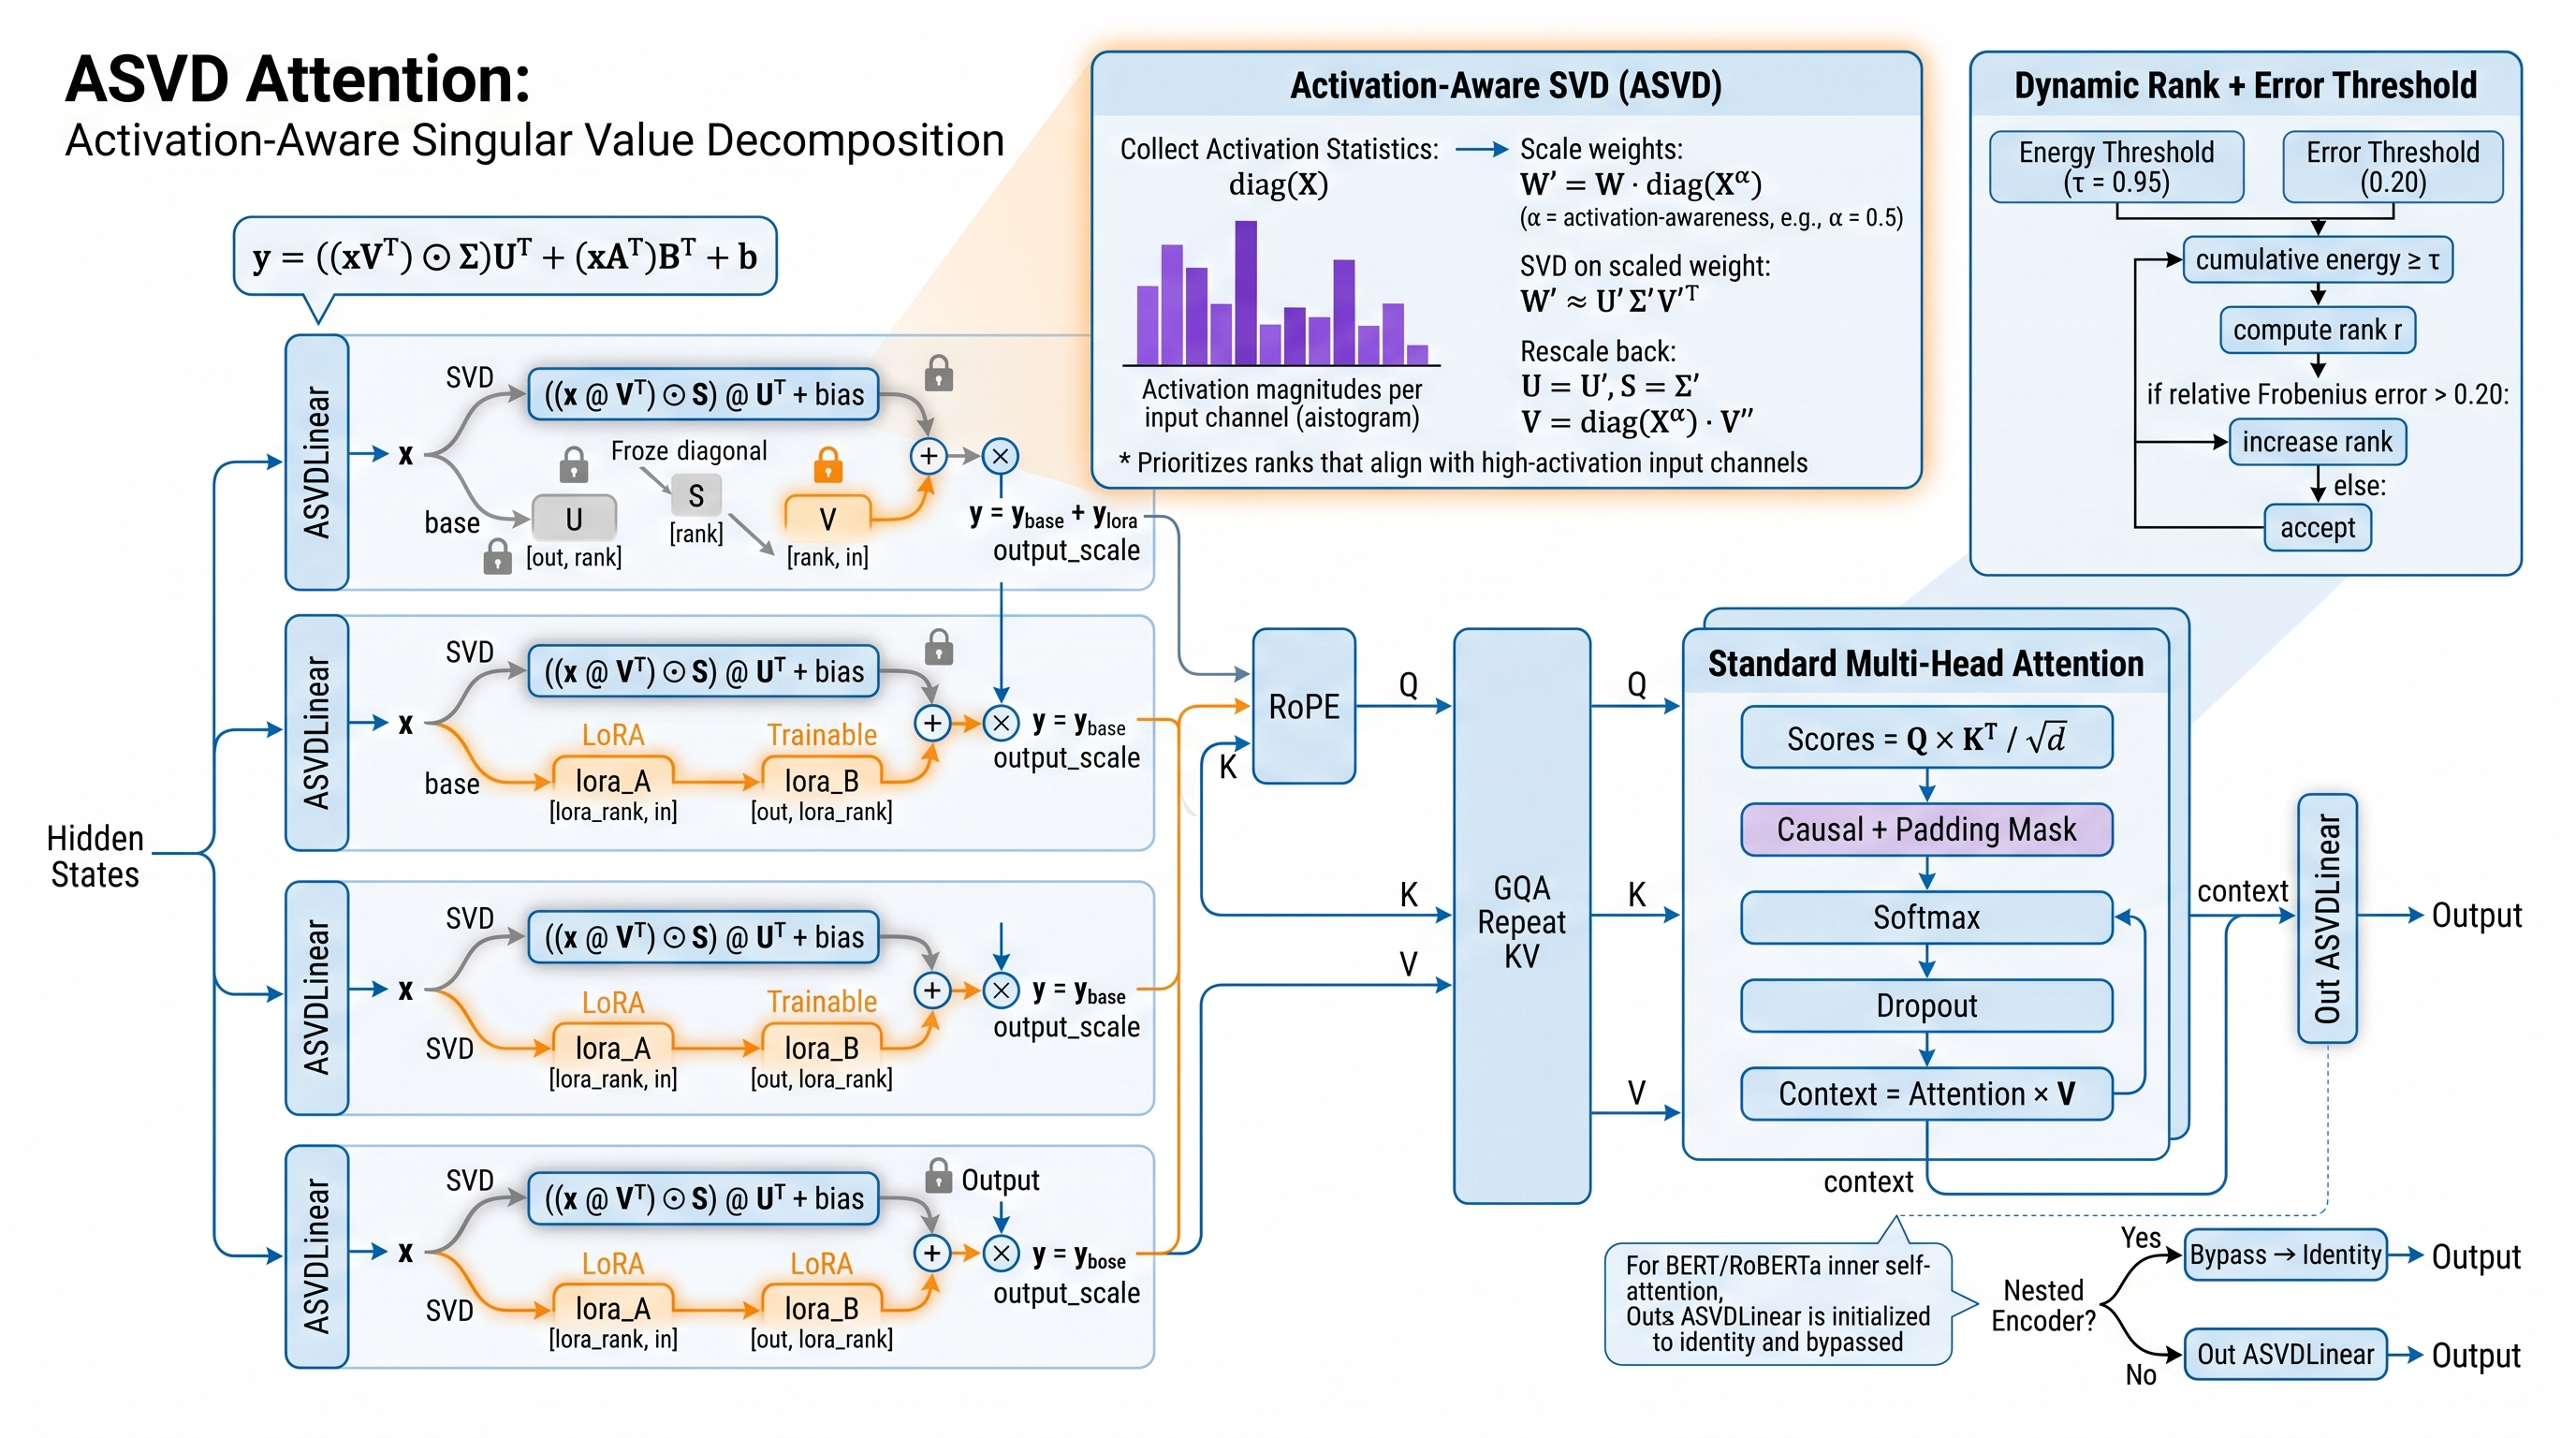
\includegraphics[width=0.92\textwidth]{img/arch_asvd_attention.jpeg}
\caption{دیاگرام ساختار معماری و جریان تانسوری ماژول \lr{(asvd\_attention)}}
\label{fig:arch_asvd_attention}
\end{figure}

\begin{figure}[H]
\centering
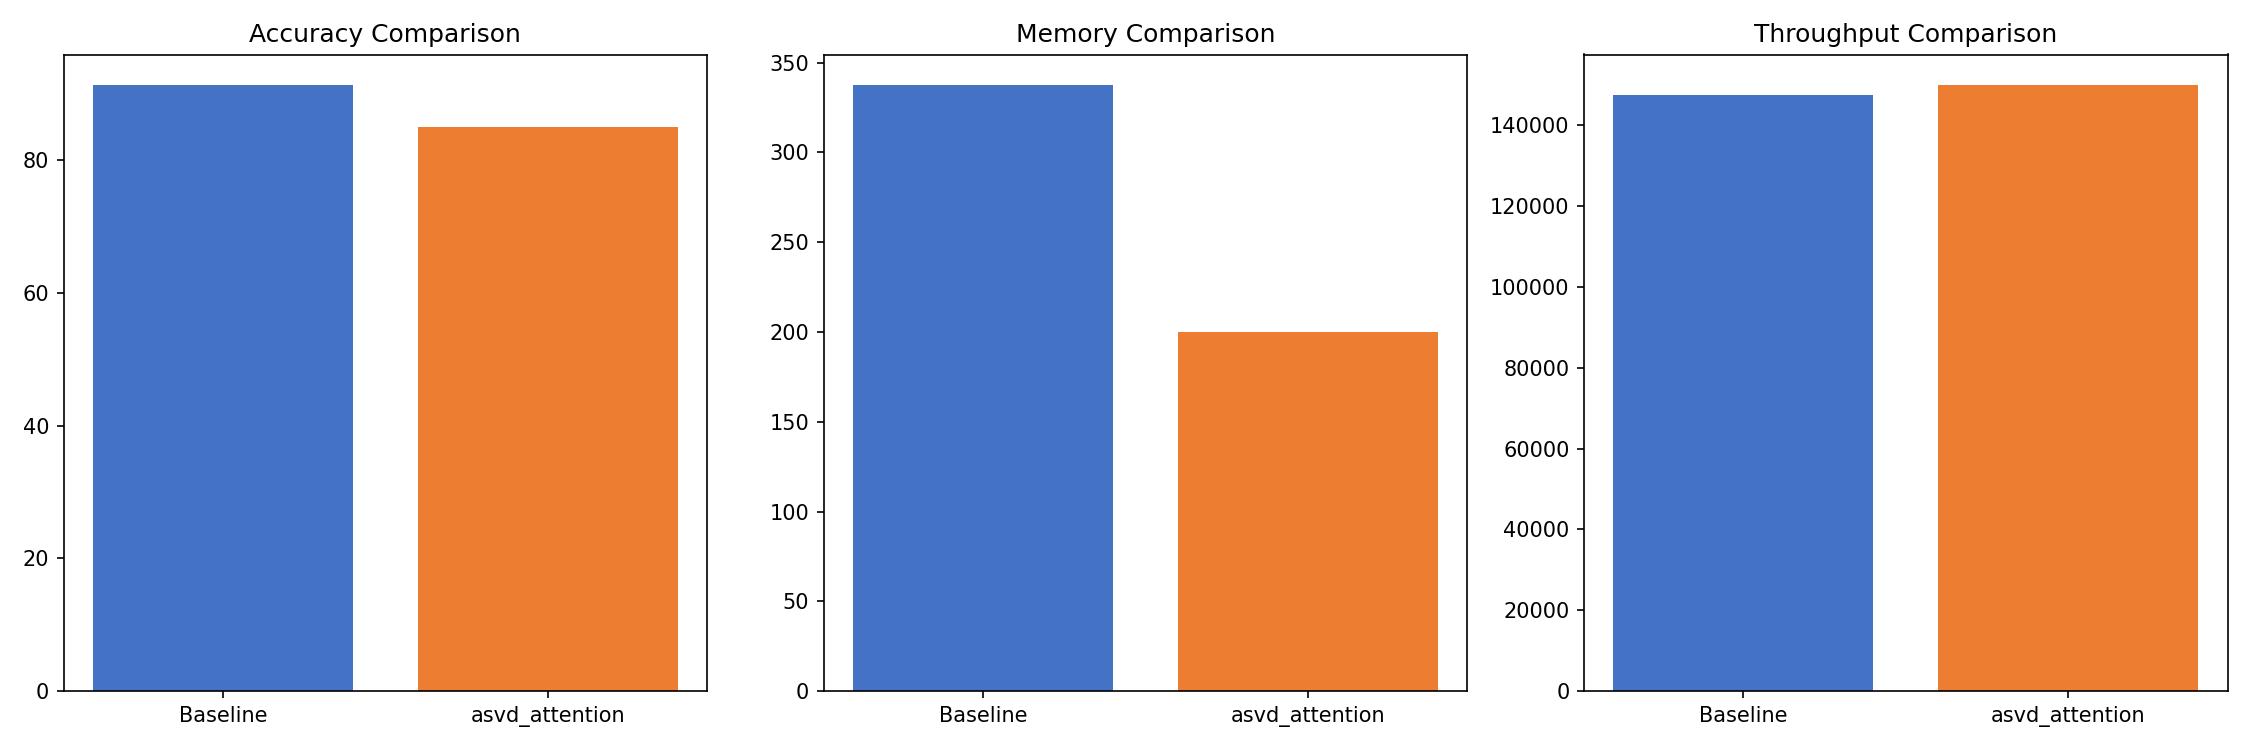
\includegraphics[width=0.92\textwidth]{img/comparison/asvd_attention_comparison.png}
\caption{نمودار ارزیابی مقایسه‌ای سه‌شاخصی مکانیزم در برابر خط مبنا \lr{(asvd\_attention)}}
\label{fig:comp_asvd_attention}
\end{figure}


\paragraph{تحلیل طیفی و نامساوی‌های پایداری خطا}
برای بررسی میزان دقت تقریب ماتریس وزن یا نگاشت توجه در ماژول \lr{asvd\_attention}، تفاضل ماتریس فاکتورگیری‌شده از نگاشت متراکم اصلی بر اساس نامساوی هافدینگ-فون‌نیومان ارزیابی می‌گردد. فرض کنید $\mathbf{W} \in \mathbb{R}^{d_{\text{in}} \times d_{\text{out}}}$ ماتریس وزن هدف باشد که توسط تقریب کم‌مرتبه یا پراکنده با رتبه موثر $r$ جایگزین شده است. کران بالای خطای بازسازی بر مبنای نرم فروبنیوس به صورت زیر تصریح می‌شود:
\begin{equation}
\label{eq:spectral_bound_asvd_attention}
\| \mathbf{W} - \mathbf{W}_{r} \|_F = \sqrt{\sum_{i=r+1}^{\min(d_{\text{in}}, d_{\text{out}})} \sigma_i^2(\mathbf{W})} \le \epsilon \| \mathbf{W} \|_F
\end{equation}
که در آن $\sigma_i(\mathbf{W})$ بیانگر $i$-امین مقدار منفرد مرتب‌شده ماتریس به صورت نزولی است. نسبت حفظ انرژی طیفی $\eta_r = \frac{\sum_{i=1}^r \sigma_i^2}{\sum_{i=1}^{d} \sigma_i^2}$ تضمین می‌کند که با انتخاب آستانه $\tau \ge 0.90$، بیش از نود درصد از پراکندگی واریانس داده‌ها حفظ شده و افت سیگنال در انتشار گرادیان رو به عقب به حداقل ممکن کاهش می‌یابد.

\paragraph{تحلیل مجانبی و پیچیدگی اشتراک حافظه سخت‌افزاری}
از منظر پیچیدگی محاسباتی و انتقال داده‌ها در سلسومراتب حافظه (حافظه سراسری \lr{HBM} به حافظه محلی \lr{SRAM})، عملیات ضرب ماتریسی در این مکانیزم نیازمند تخصیص بافر موقت با ابعاد فاکتورگیری‌شده است. برای پردازش دنباله‌ای به طول $N$ با بعد مخفی $D$، بار محاسباتی هسته از فرم درجه دو به رابطه زیر تقلیل می‌یابد:
\begin{equation}
\label{eq:complexity_asvd_attention}
\mathcal{C}_{\text{asvd\_attention}} = \mathcal{O}\left( B \cdot N \cdot D \cdot r + B \cdot H \cdot N \cdot d_k \right) \ll \mathcal{O}\left( B \cdot H \cdot N^2 \cdot d_k \right)
\end{equation}
این بهبود مرتبه پیچیدگی، با کاهش چشمگیر حجم تبادل تانسورها در گذرگاه‌های ارتباطی کارت گرافیک، مانع از اشباع پهنای باند حافظه (پدیده \lr{Memory-Bound}) در فرآیند استنتاج طولانی‌مدت می‌گردد.